\subsection{Loss Functions}
The purpose of loss functions, also known as cost functions, is to measure the discrepancy between the predicted output of the network and the true target variable, guiding the parameter optimization process.
Various functions can be defined based on the type of problem.

\subsubsection{Classification}
\begin{itemize}
    \item \textbf{Cross-Entropy Loss}: used for multi-class classification problems. 
    It measures the dissimilarity between the predicted probability of class $\hat{y}_i$ and the true class label.
    For a single data point, the loss can be expressed as:
    \begin{equation*}
        \loss(y, \hat{y}) = -\sum_{i=1}^{C} y_i \log(\hat{y}_i)
    \end{equation*}
    where $C$ is the number of classes, $y_i$ is the true label (one-hot encoded), and $\hat{y}_i$ is the predicted probability for class $i$.
    
    \item \textbf{Binary Cross-Entropy Loss}: special case of the categorical cross-entropy loss for binary classification problems.
    For a single data point, the loss can be expressed as:
    \begin{equation*}
        \loss(y, \hat{y}) = -[y \log(\hat{y}) + (1 - y) \log(1 - \hat{y})]
    \end{equation*}
\end{itemize}

\subsubsection{Regression}
\begin{itemize}
    \item \textbf{Mean Squared Error (MSE)}: commonly used for regression problems. 
    It measures the average squared difference between the predicted and true values.
    For a single data point, the loss can be expressed as:
    \begin{equation*}
        \loss(y, \hat{y}) = \frac{1}{2}(y - \hat{y})^2
    \end{equation*}
    The squared term ensures that the function is convex (easy to optimize), but penalizes larger errors more than smaller ones, as the difference is squared.
    This causes the loss function to be sensitive to outliers in the data, as they can have a disproportionate influence on the overall loss.

    \item \textbf{Mean Absolute Error (MAE)}: similar to MSE but uses the absolute difference instead of the squared difference.
    For a single data point, the loss can be expressed as:
    \begin{equation*}
        \loss(y, \hat{y}) = |y - \hat{y}|
    \end{equation*}
    This one penalizes large errors less than MSE, making it more robust to outliers.
    
    \item \textbf{Huber Loss}: combines the properties of MSE and MAE. It behaves like MSE for small errors and like MAE for large errors, providing a balance between sensitivity to outliers and smoothness of the loss function.
    Formally, for a single data point, the loss can be expressed as:
    \begin{equation*}
        \loss(y, \hat{y}) = \begin{cases}
        \frac{1}{2}(y - \hat{y})^2 & \text{for } |y - \hat{y}| \leq \delta \\
        \delta (|y - \hat{y}| - \frac{1}{2}\delta) & \text{for } |y - \hat{y}| > \delta
        \end{cases}
    \end{equation*}
    where $\delta$ is a hyperparameter that determines the threshold between the MSE and MAE behavior.
\end{itemize}
Many more loss functions exist, and can be tryed out based on the specific problem and data characteristics.

\subsubsection{Contrastive Learning}
Another branch that is worth mentioning is the one used to train models in a self-supervised way, such as contrastive learning.
As shown in the figure \ref{fig:left}, the idea is to learn a representation of the data that captures the underlying structure and relationships between data points,
that is invariant to certain transformations.

The loss function used in contrastive learning is designed to encourage the model to learn representations that are similar for similar data points and dissimilar for different data points.
A possible loss function for contrastive learning is the \textbf{Noise Contrastive Estimation} (NCE) loss, which can be expressed as follows:
\begin{equation*}
    NCE_{Loss} = -\log \frac{e^{\simop(\vct{z}_i, \vct{z}_j)}}
    {e^{\simop(\vct{z}_i, \vct{z}_j)} + \sum_{k=1}^{N} e^{\simop(\vct{z}_i, \vct{z}_k)}}
\end{equation*}
where $\vct{z}_i$ and $\vct{z}_j$ are the representations of two similar data points (anchor and positive), $\vct{z}_k$ are the representations of all data points (negatives), 
$\simop(\cdot, \cdot)$ is a similarity function (e.g., cosine similarity). 
\begin{figure}[H]
    \centering
    \begin{minipage}{0.45\textwidth}
        \centering
        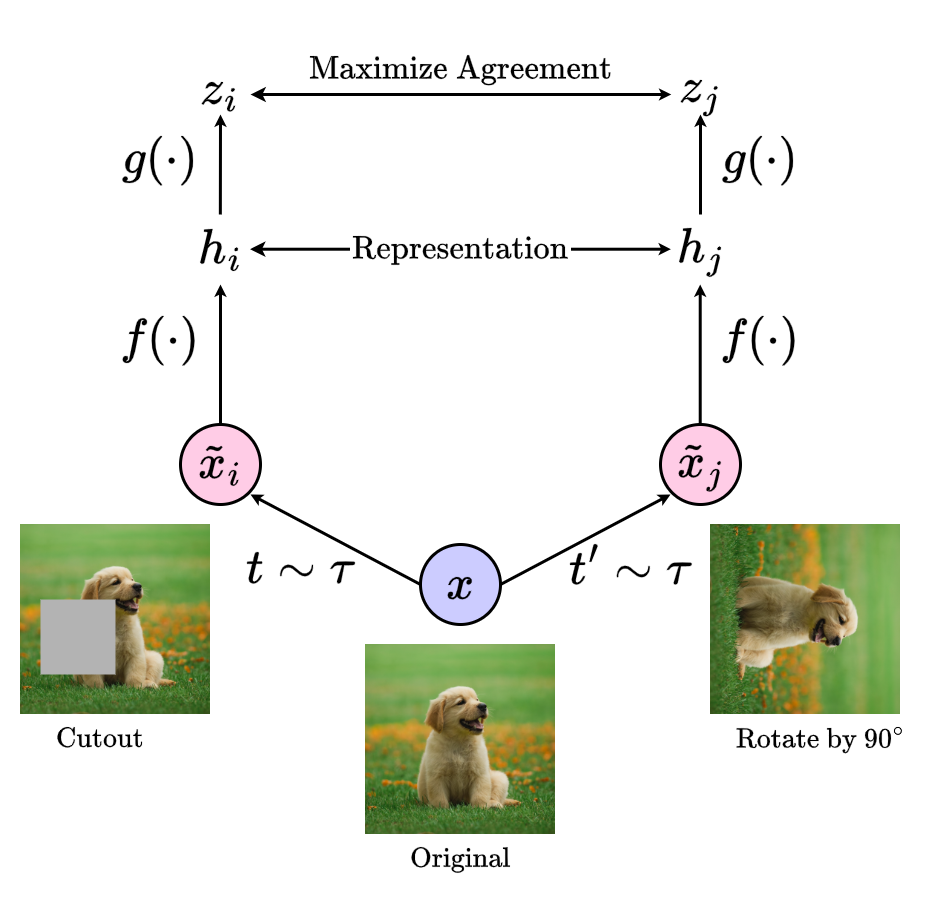
\includegraphics[width=\textwidth]{chapters/02-ffnn/media/contrastive_learning.png}
        \caption{Contrastive learning Model}
        \label{fig:left}
    \end{minipage}
    \hfill
    \begin{minipage}{0.45\textwidth}
        \centering
        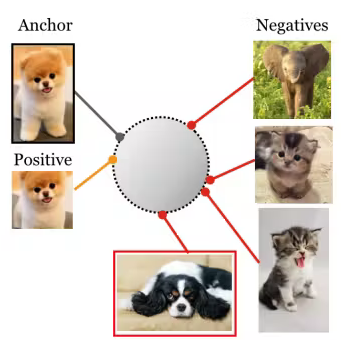
\includegraphics[width=\textwidth]{chapters/02-ffnn/media/contrastive_learning_1.png}
        \caption{Contrastive learning loss function}
        \label{fig:right}
    \end{minipage}
\end{figure}